\documentclass[12pt,a4paper,oneside]{report}

% ----------------------------------------------------------------------
% Packages
% ----------------------------------------------------------------------
\usepackage[utf8]{inputenc}
\usepackage[T1]{fontenc}
\usepackage[margin=2.5cm]{geometry}
\usepackage{setspace}
\usepackage{graphicx}
\usepackage{booktabs}
\usepackage{caption}
\usepackage{amsmath}
\usepackage{amssymb}
\usepackage{fancyhdr}
\usepackage[hidelinks]{hyperref}
\usepackage[nameinref]{cleveref}

% ----------------------------------------------------------------------
% Layout
% ----------------------------------------------------------------------
\onehalfspacing
\setcounter{secnumdepth}{3}
\setcounter{tocdepth}{2}

\pagestyle{fancy}
\fancyhf{}
\fancyhead[L]{\nouppercase{\leftmark}}
\fancyfoot[C]{\thepage}
\renewcommand{\headrulewidth}{0.4pt}

% ----------------------------------------------------------------------
% Title page details -- edit these for your submission
% ----------------------------------------------------------------------
\newcommand{\thesistitle}{Automatic Plain-Language Simplification of Public-Facing Health Information Using Transformer-Based NLP}
\newcommand{\thesisauthor}{Nnamdi Salau-John}
\newcommand{\thesisid}{B01037764}
\newcommand{\thesisdept}{School of Computing, Ulster University}
\newcommand{\thesismodule}{COM748}
\newcommand{\thesisdate}{\today}

\title{\thesistitle}
\author{\thesisauthor}
\date{\thesisdate}

\begin{document}

% ----------------------------------------------------------------------
% Front matter
% ----------------------------------------------------------------------
\pagenumbering{roman}

\begin{titlepage}
    \centering
    \vspace*{2cm}

    {\Large \thesisdept \par}
    \vspace{0.5cm}
    {\large \thesismodule \ -- Dissertation \par}

    \vspace{3cm}
    {\huge \bfseries \thesistitle \par}

    \vspace{2cm}
    {\large \thesisauthor \par}
    {\large Student ID: \thesisid \par}

    \vfill

    {\large \thesisdate \par}

\end{titlepage}

\chapter*{Abstract}
\addcontentsline{toc}{chapter}{Abstract}

Health information written for a general audience is often too dense for the people who need it most. Patient leaflets, treatment summaries, and public health updates frequently carry the phrasing of a clinical abstract rather than the plain language a worried reader can act on. This project asks whether a transformer-based language model can close some of that gap: can it rewrite technical biomedical text into something easier to read, without quietly dropping the details that make the information medically useful?

The work is built around Cochrane-auto, a dataset that pairs sentences from Cochrane systematic review abstracts with their official plain-language summaries. A small transformer, T5-small, was fine-tuned on these pairs and compared against two baselines: a hand-written rule-based simplifier and the same T5-small model used without any fine-tuning. All three systems were evaluated on a held-out test sample using established readability formulas (Flesch Reading Ease, Flesch-Kincaid Grade Level, SMOG), text generation metrics (BLEU, ROUGE), a simplification-specific metric (SARI), and a semantic similarity measure (BERTScore), followed by a manual reading of individual outputs.

Fine-tuning clearly helped relative to the untrained model. The zero-shot T5-small often produced disfluent or even non-English text, while the fine-tuned version reliably returned coherent sentences and scored well ahead of it on every metric. Against the simpler rule-based baseline the picture was more mixed: the fine-tuned model edged ahead on SARI, ROUGE, and BERTScore, but the rule-based system, and even the untouched source text, sometimes scored as more readable by the surface-level formulas. Manual inspection suggested why. At the training scale used here, the model tends to make small, safe edits, such as removing a statistical parenthetical, rather than the kind of restructuring a human writer produces when a sentence needs deeper rephrasing. In several cases the reference summary answers a slightly different question than the source sentence poses, which is itself a property of the dataset worth flagging for anyone building on this work.

The result is a working, reproducible simplification pipeline rather than a finished product, and the thesis is explicit about that. It documents where automation already helps, where it currently falls short, and why a health-communication tool built this way still needs a human in the loop before it goes near a real patient.


\tableofcontents
\clearpage
\listoffigures
\clearpage
\listoftables
\clearpage

% ----------------------------------------------------------------------
% Main matter
% ----------------------------------------------------------------------
\pagenumbering{arabic}

\chapter{Introduction}
\label{ch:introduction}

\section{Motivation}
\label{sec:motivation}

Most people encounter health information at the exact moment they are least equipped to parse dense writing: after a diagnosis, before a procedure, or while trying to make sense of a public health notice that affects their family. The text they are handed, whether a patient leaflet, a treatment explanation, or a summary of new research, is often written by and for people with clinical training. Long sentences, specialist vocabulary, and formal phrasing are the norm rather than the exception, even when the stated purpose of the document is to inform the public~\cite{hra2025plainlanguage,mrct2025plainlanguage}.

This is not simply a matter of style. When a person cannot follow what a piece of health information is actually telling them, the consequences extend to how confidently they make decisions, whether they follow medical advice, and how much they trust the healthcare system in general. Text simplification, the task of rewriting a passage so that it is easier to read while keeping its meaning intact, offers one route to narrowing that gap. Progress in transformer-based natural language processing over the past several years has made automatic simplification a realistic option rather than a research curiosity, but taking a model built for open-domain text and pointing it at biomedical writing is not guaranteed to work. Clinical text carries a kind of precision that ordinary prose does not: a hedge like ``may reduce the risk'' is not there by accident, and a model that smooths it into ``reduces the risk'' has changed the claim, not just the wording.

This project sits at that intersection. It uses Cochrane-auto, a dataset built specifically to align technical abstracts with their official plain-language counterparts, to fine-tune a small transformer model for health text simplification, and it treats the risk of losing meaning as seriously as the goal of improving readability.

\section{Problem Statement}
\label{sec:problem-statement}

Public-facing health and social care information is frequently written above the reading level of the people it is meant to serve. A person handed a leaflet about a diagnosis or a treatment option may struggle to extract what it actually means for them, not because the information is unavailable, but because the sentences are long, the terminology is specialised, and the tone is more formal than the situation calls for.

This dissertation investigates whether a transformer-based simplification system can rewrite that kind of text into something clearer, without stripping out the medical substance that made the original worth reading in the first place. The question matters because misunderstanding health information carries real consequences for decision-making, adherence to treatment, and access to care more broadly. Existing simplification systems already show promise on general text, but recent work suggests that biomedical and health content needs its own training data rather than a transfer from encyclopaedic or news-based corpora, since the risk of quietly distorting a clinical claim is much higher here than in most other simplification settings~\cite{bakker2024cochraneauto,zhang2020bertscore}.

\section{Research Question}
\label{sec:research-question}

Can transformer-based text simplification improve the readability of public-facing health information while preserving its original meaning?

\section{Aim and Objectives}
\label{sec:aims-objectives}

\subsection*{Aim}

To design, implement, and evaluate a transformer-based plain-language simplification pipeline for health-related text, with particular attention to whether readability gains come at the cost of meaning.

\subsection*{Objectives}

\begin{enumerate}
    \item Prepare a clean, paired dataset of complex biomedical sentences and their simplified counterparts, using Cochrane-auto as the primary source.
    \item Implement a simple, non-learned baseline for comparison, combining rule-based sentence splitting with conservative lexical substitution.
    \item Fine-tune a compact transformer model, T5-small, on the prepared dataset, and compare it against the same model used without fine-tuning.
    \item Evaluate every system using readability formulas, overlap-based text generation metrics, a simplification-specific metric, and a semantic similarity measure.
    \item Carry out a manual reading of individual outputs to check what the automatic metrics might be missing.
    \item Discuss where the pipeline succeeds, where it fails, and what that implies for using automatic simplification in a health communication context.
\end{enumerate}

\section{Thesis Structure}
\label{sec:thesis-structure}

\Cref{ch:literature-review} reviews the text simplification literature relevant to this project, from general-domain datasets through to the biomedical resources this work is built on. \Cref{ch:dataset} describes the Cochrane-auto dataset and the exploratory analysis carried out before any modelling began. \Cref{ch:data-preparation} covers how the raw aligned data was cleaned and turned into training pairs. \Cref{ch:methodology} sets out the two baseline systems and the fine-tuning procedure used for the main model. \Cref{ch:evaluation-methodology} defines the metrics used to judge the outputs, including the formulas behind each one. \Cref{ch:results-discussion} reports the results and discusses what they mean, supported by a manual reading of individual examples. \Cref{ch:conclusion} closes with the limitations of the current work, the ethical considerations that shaped its design, and directions for extending it further.

\chapter{Literature Review}
\label{ch:literature-review}

\section{Plain Language and the Case for Simplification}
\label{sec:plain-language}

Health literacy research rarely frames clarity as a vague virtue. It points to specific, checkable choices: shorter sentences, everyday vocabulary, an explicit statement of risk, and honest signalling of uncertainty rather than false confidence~\cite{hra2025plainlanguage,mrct2025plainlanguage}. Text simplification research arrives at the same territory from a different direction. Instead of starting from health communication practice, it treats simplification as a rewriting task: take a complex passage and produce an easier one that says roughly the same thing.

Older simplification systems often handled this as a single operation performed in isolation, substituting a word here or deleting a clause there. More recent work treats it as something messier. A good simplification might split a long sentence, replace a technical term, reorder two clauses, and drop a piece of non-essential detail, all within the same rewrite~\cite{alvamanchego2020asset}. Health text raises the stakes on every one of those decisions. A sentence describing a treatment's side effects or a trial's statistical uncertainty cannot be shortened without thinking about what the shortening removes. Swapping a technical phrase for a simpler one might genuinely help a reader. It might just as easily blur a distinction the original author meant to preserve. That tension is the reason this project treats health text as a domain of its own rather than an extension of general-purpose simplification.

\section{Cochrane-auto and Domain-Specific Supervision}
\label{sec:cochrane-auto-lit}

The strongest justification for this project's design comes from Cochrane itself. Cochrane systematic reviews are already published with two versions: a technical abstract for researchers and clinicians, and a plain-language summary written for the public. Bakker and Kamps formalised this existing practice into a dataset, Cochrane-auto, by aligning the two versions at sentence, paragraph, and document level using a trained alignment model~\cite{bakker2024cochraneauto}. That distinction matters for this project because it supplies genuine, domain-specific training data rather than forcing reliance on simplification examples drawn from Wikipedia or news writing, neither of which resembles clinical prose.

Cochrane-auto's multi-level alignment opens several ways to frame the modelling task. A project with limited time and computing resources is more likely to succeed working at the sentence or short-paragraph level, and that is the scope adopted here. The dataset also raises a broader question that resurfaces throughout this thesis: whether acceptable health simplification is really a sentence-by-sentence rewriting problem, or whether it depends on coherence across a whole explanation in a way that sentence-level training cannot capture. Bakker and Kamps report that a system trained on their aligned data outperformed a baseline trained on unaligned technical and lay text, which supports the idea that alignment quality drives simplification quality in this domain. It is worth being careful with that finding, though. A model that scores well on automatic metrics has not necessarily learned to explain a screening result, a medication risk, or a treatment benefit in a way a patient can actually use. It may simply have learned the surface style of a lay summary.

\section{What General-Domain Datasets Still Offer}
\label{sec:general-domain-datasets}

Cochrane-auto is the primary training resource in this project, but the wider simplification literature still shapes how the results are interpreted. ASSET is a useful reminder that simplification rarely reduces to one clean edit. Each source sentence in ASSET is paired with several independent human rewrites, and those rewrites differ in how they combine splitting, paraphrasing, deletion, and restructuring~\cite{alvamanchego2020asset}. That variation matters for evaluation as much as for training. Judge a simplification against a single reference and a perfectly reasonable rewrite can look worse than it is, simply because it took a different but equally valid path. ASSET is treated here as a comparison and calibration resource rather than a training set, since it reflects general writing rather than the clinical register this project is concerned with.

WikiAuto contributes a different lesson. Jiang et al.\ showed that the quality of sentence alignment has a direct effect on the quality of any simplification model trained on that alignment~\cite{jiang2020wikiauto}. That sounds close to self-evident once stated, but it carries a sharper edge in a health context: poor alignment does not just add noise to training. It risks teaching a model the wrong relationship between a technical claim and its plain-language explanation, which is a mistake far more consequential in medicine than in encyclopaedic writing.

\section{Evaluating Simplification, and the Limits of Doing So Automatically}
\label{sec:evaluation-lit}

Evaluation in this field carries a persistent discomfort, and it probably should. BLEU remains the most familiar metric largely because of its origins in machine translation, but it was never built to measure simplicity~\cite{papineni2002bleu}. A model can produce a genuinely clearer sentence, phrase it differently from the reference, and be penalised for low word overlap regardless. ROUGE has a related limitation: it can say something about how much content survived the rewrite, but nothing about whether the result is actually easier to read~\cite{lin2004rouge}.

SARI was designed specifically to address this gap. It scores a simplification by how well it adds, keeps, and deletes words relative to the source and one or more references, which fits the task far better than a translation metric repurposed for a different job~\cite{xu2016sari}. Even so, SARI is not a complete answer. Surface readability formulas such as Flesch Reading Ease, Flesch-Kincaid Grade Level, and SMOG can indicate whether an output looks simpler, but none of them can confirm that the sentence is accurate, safe, or natural to read. Recent work on meaning preservation makes this point directly: simplification systems can score well on every automatic measure available while still distorting meaning in ways a human reader would notice immediately~\cite{meaningpreservation2024tacl}. In a health context, a subtle shift, softening a hedge, dropping a qualifier, changing the strength of a recommendation, is not a minor stylistic slip. It can change what a reader takes away from the text. Semantic similarity measures such as BERTScore, which compare candidate and reference text using contextual embeddings rather than surface overlap, offer one way to catch some of this drift, and this project uses BERTScore alongside SARI, BLEU, and ROUGE for exactly that reason~\cite{zhang2020bertscore}.

\section{Transformer Models in Simplification Research}
\label{sec:transformers-lit}

Transformer-based encoder-decoder models now dominate the practical side of text simplification, largely because a single architecture can learn paraphrasing, compression, and restructuring together rather than needing separate rule sets for each~\cite{vaswani2017attention}. T5 and BART are attractive choices for a project like this one because they are documented, widely used, and small enough to fine-tune without specialised hardware~\cite{raffel2020t5,lewis2020bart}. Choosing a compact variant such as T5-small over a larger model is a deliberate trade-off rather than a limitation to apologise for. A smaller model is easier to fine-tune and easier to interpret. If it performs well, the result is straightforward to explain. If it struggles, the reasons are easier to trace than they would be inside a much larger system.

Recent work applying large language models to biomedical and lay summarisation repeats a consistent warning: readability improvement is only one part of the task, and factual stability under simplification is much harder to secure~\cite{llmbiomedsimplification2024}. That caution shapes the design of this project directly. Automatic gains in readability are not treated here as evidence of success on their own.

\section{Human Variation and Document-Level Coherence}
\label{sec:variation-coherence}

Human writers do not simplify text the same way twice. Some explain a concept before shortening it. Others cut aggressively first and clarify afterwards. Some keep a technical term and gloss it in place, while others replace it outright. Studies of this variability suggest that trained models tend to produce narrower, more repetitive rewrites than human writers do~\cite{variability2024tsar}, which in a health context risks text that is technically simpler but strangely generic, stripped of the nuance a human writer would have kept.

Coherence across several sentences matters more than sentence-level benchmarks usually acknowledge. A patient information page is not a bag of independently simplified sentences. It carries a line of reasoning, sometimes a warning, that only makes sense read in sequence, and document-level simplification work has begun to take that seriously~\cite{documentlevel2023tsar}. This project works at sentence level for practical reasons, but the evaluation in \cref{ch:results-discussion} stays alert to coherence problems that only become visible once outputs are read as connected text rather than isolated examples.

\section{Positioning of This Study}
\label{sec:positioning}

Taken together, the literature supports two claims this project relies on. Aligned biomedical simplification is feasible with current datasets and models, and automatic evaluation on its own is not enough to trust the result~\cite{bakker2024cochraneauto,alvamanchego2020asset,jiang2020wikiauto}. There is still room for smaller, carefully scoped studies that ask a narrower question than most of the literature attempts: can a modest transformer model, fine-tuned on a realistic amount of health-domain data, improve readability without quietly damaging the meaning a reader depends on. Reinforcement-learning approaches to simplification have also been explored for accessibility purposes outside the health domain~\cite{baggio2025rl}, though this project takes a supervised fine-tuning approach in keeping with the scale of data and compute available.

This project does not assume simplification is automatically beneficial, and it does not treat over-simplification as a hypothetical risk either. Both possibilities are taken seriously, and the results in \cref{ch:results-discussion} are reported with that balance in mind.

\chapter{Dataset}
\label{ch:dataset}

\section{Dataset Selection}
\label{sec:dataset-selection}

The main dataset used in this project is Cochrane-auto~\cite{bakker2024cochraneauto}, an aligned corpus that pairs sentences from Cochrane systematic review abstracts with their official plain-language summaries. It was chosen over general-domain simplification datasets because it puts the project's central question, whether a model can simplify health text without losing medical substance, directly at the centre of the training data rather than treating it as an afterthought.

ASSET and WikiAuto were considered as alternatives but kept to a supporting role. ASSET is a multi-reference sentence simplification dataset built from encyclopaedic text, useful for understanding how evaluation against multiple references works, but not representative of clinical writing~\cite{alvamanchego2020asset}. WikiAuto is similarly built on Wikipedia-style prose and carries stylistic habits that do not transfer cleanly to patient-facing health content~\cite{jiang2020wikiauto}. Both remain useful as comparison points rather than as training data for this project.

\section{Acquisition}
\label{sec:acquisition}

Cochrane-auto is distributed with the code used to build it, together with pre-computed sentence-level, paragraph-level, and document-level versions of the aligned data, already split into training, validation, and test sets. This project uses the published split throughout rather than constructing a new one, both to avoid accidentally leaking test examples into training and to keep any later comparison against the original paper straightforward.

Modelling in this project works at sentence level. Cochrane abstracts and their lay summaries can run to several hundred words, and full paragraph or document-level training would demand longer sequence lengths and considerably more compute than a project of this scale can commit to. Sentence-level pairs keep the task tractable for a compact model such as T5-small while still capturing the core rewriting behaviour this project is interested in.

\section{Structure of the Aligned Data}
\label{sec:data-structure}

Each row in the sentence-level data links one sentence from a technical abstract to zero or more sentences from the corresponding lay summary. Every row carries a label describing the type of rewrite that connects the two, produced by the alignment model used to build Cochrane-auto. \Cref{tab:alignment-labels} summarises what each label means and how it was used in this project.

\begin{table}[htbp]
    \centering
    \caption{Rewrite-operation labels in the Cochrane-auto sentence-level data.}
    \label{tab:alignment-labels}
    \begin{tabular}{@{}ll@{}}
        \toprule
        \textbf{Label} & \textbf{Meaning} \\
        \midrule
        \texttt{rephrase} & The technical sentence maps to a single simplified sentence. \\
        \texttt{split} & Its content is spread across more than one simplified sentence. \\
        \texttt{merge} & It is combined with other sentences into one simplified sentence. \\
        \texttt{delete} & The sentence was dropped entirely from the lay summary. \\
        \texttt{ignore} / \texttt{none} & No reliable alignment could be established. \\
        \bottomrule
    \end{tabular}
\end{table}

Training pairs for this project were built from every row with a non-empty simplified target, which naturally keeps \texttt{rephrase} and \texttt{split} rows and the contributing row of a \texttt{merge} group, while correctly leaving out sentences that were deleted or never reliably aligned. In the training split, 5{,}239 sentences were tagged \texttt{rephrase}, 521 \texttt{split}, and 365 \texttt{merge}, against 4{,}063 tagged \texttt{delete} and 1{,}322 tagged \texttt{ignore} or \texttt{none}. \Cref{fig:label-distribution} shows how these counts break down across the training, validation, and test splits.

\begin{figure}[htbp]
    \centering
    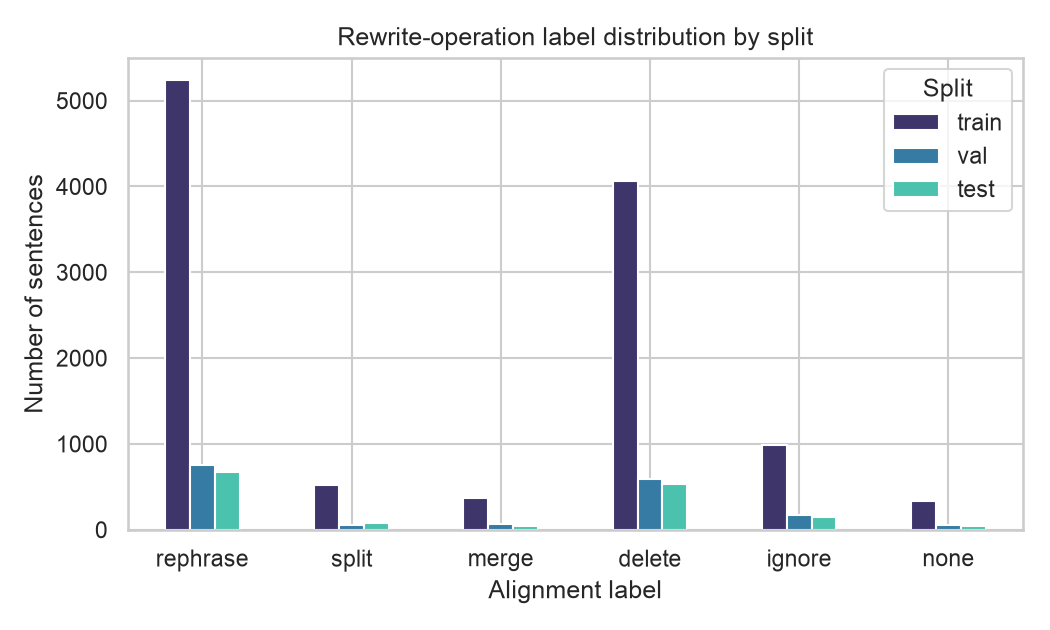
\includegraphics[width=0.85\textwidth]{figures/01_label_distribution.png}
    \caption{Rewrite-operation label distribution across the train, validation, and test splits.}
    \label{fig:label-distribution}
\end{figure}

\section{Exploratory Analysis}
\label{sec:eda}

Before any modelling took place, the extracted pairs were examined for sentence length, the degree to which the simplified version compresses or expands the original, and a manual reading of a sample from each label category. This step matters beyond simple description: it shapes what counts as a fair baseline and what kind of model error is worth taking seriously later in the project.

\Cref{tab:eda-summary} reports descriptive statistics for the 7{,}082 training pairs with a non-empty simplified target. The compression ratio is the simplified sentence's word count divided by the complex sentence's word count, so a value below one means the plain-language version is shorter.

\begin{table}[htbp]
    \centering
    \caption{Descriptive statistics for training pairs (word counts and compression ratio).}
    \label{tab:eda-summary}
    \begin{tabular}{@{}lrrr@{}}
        \toprule
         & \textbf{Complex (words)} & \textbf{Simple (words)} & \textbf{Compression ratio} \\
        \midrule
        Mean   & 24.86 & 23.59 & 1.13 \\
        Std.\ dev. & 15.66 & 12.88 & 0.72 \\
        Minimum & 1     & 3     & 0.06 \\
        25th percentile & 15 & 15 & 0.73 \\
        Median & 21    & 21    & 1.00 \\
        75th percentile & 31 & 29 & 1.27 \\
        Maximum & 186   & 145   & 9.75 \\
        \bottomrule
    \end{tabular}
\end{table}

The mean compression ratio of 1.13 is higher than intuition might suggest for a simplification dataset, and it points to something worth stating plainly. Cochrane lay summaries do not only shorten technical sentences. In a meaningful share of cases they are about the same length or longer than the source, because the writer has added context, defined a term, or explained why a result matters rather than simply trimming it. \Cref{fig:length-compression} shows the full length distributions and the spread of compression ratios, and \cref{fig:complex-vs-simple} plots complex sentence length against simplified sentence length directly, coloured by rewrite label.

\begin{figure}[htbp]
    \centering
    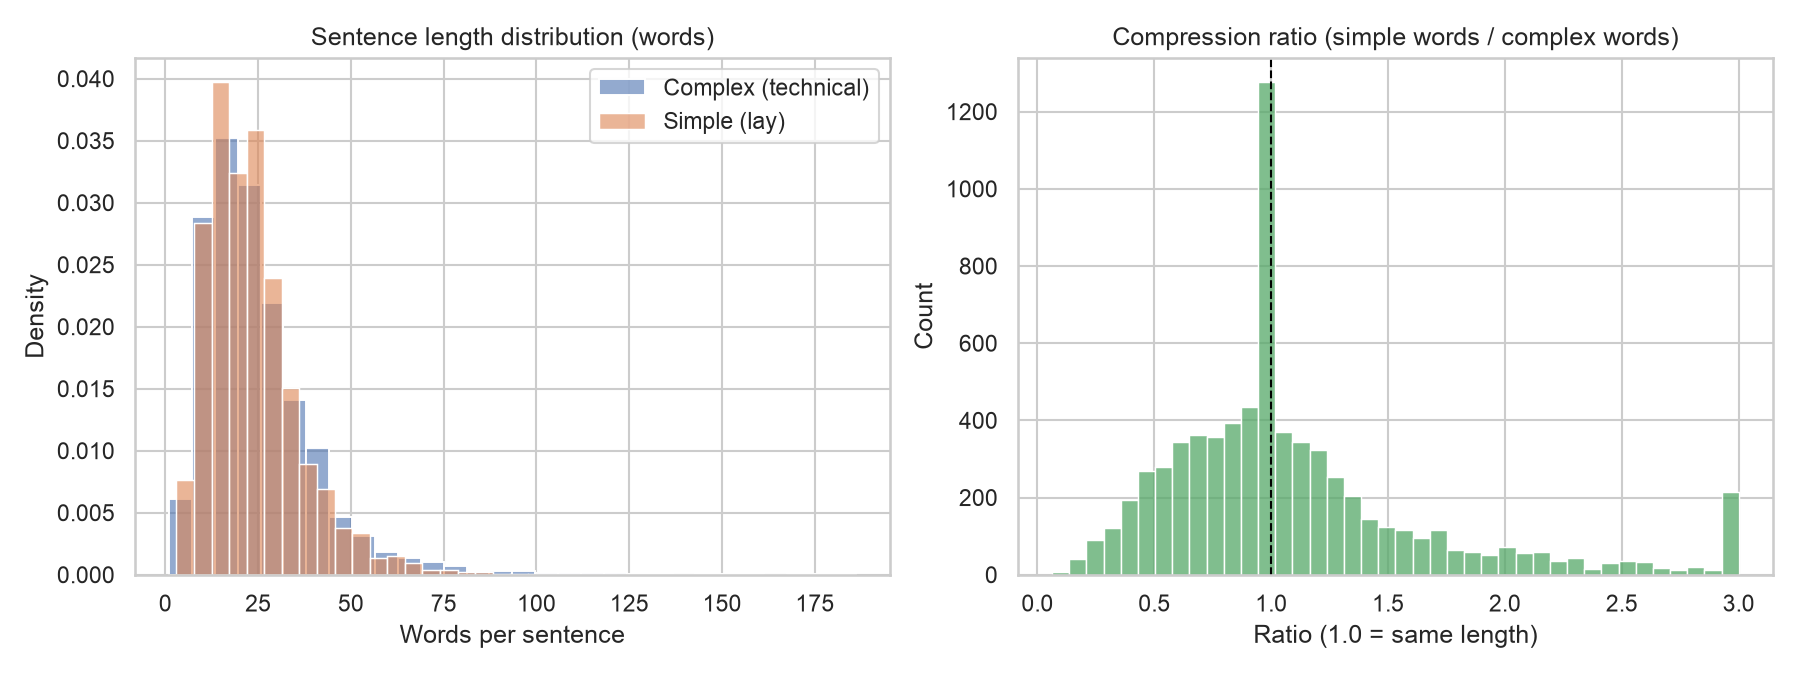
\includegraphics[width=\textwidth]{figures/02_length_and_compression.png}
    \caption{Sentence length distributions for complex and simplified text (left) and the distribution of compression ratios (right).}
    \label{fig:length-compression}
\end{figure}

\begin{figure}[htbp]
    \centering
    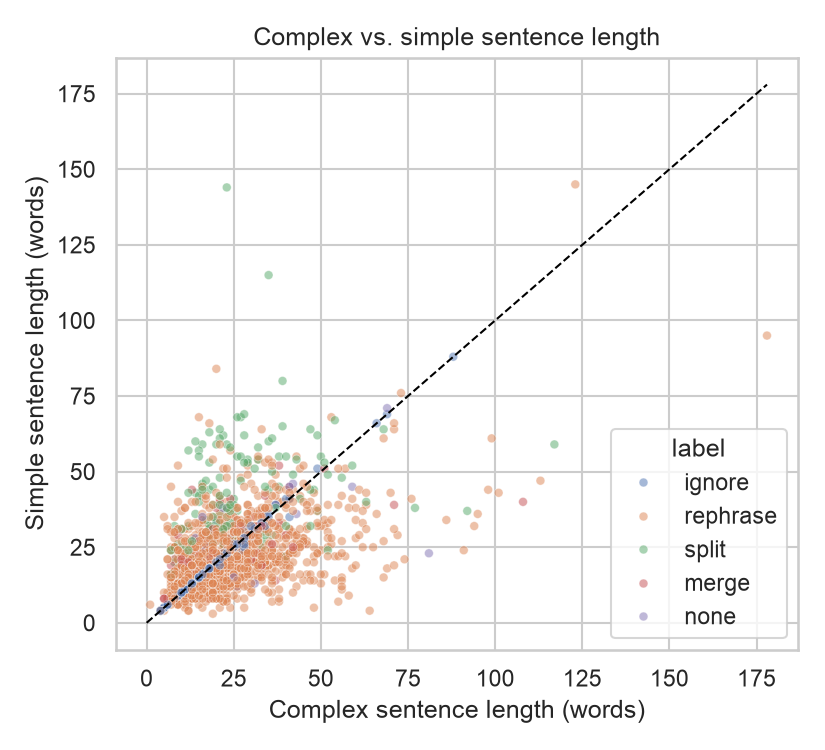
\includegraphics[width=0.75\textwidth]{figures/03_complex_vs_simple_scatter.png}
    \caption{Complex sentence length plotted against simplified sentence length, by rewrite-operation label.}
    \label{fig:complex-vs-simple}
\end{figure}

A manual reading of sample pairs from each label category reinforced this observation. Several \texttt{rephrase} pairs read as a fairly direct restatement, but a number of \texttt{split} pairs showed the lay summary adding a sentence of explanation that has no direct counterpart in the source text at all, of the kind ``this means the results should be interpreted with caution.'' That pattern suggests the task learned from this dataset is not pure sentence simplification in the narrow sense. It sits closer to a constrained form of lay summarisation, where the model is expected to compress, clarify, and occasionally explain, all within a single rewrite. That framing carries through the rest of this thesis, including the discussion of results in \cref{ch:results-discussion}, where some of the model's apparent underperformance turns out to reflect this mismatch between what the source sentence says and what the reference summary was actually written to communicate.

\chapter{Data Preparation}
\label{ch:data-preparation}

\section{Guiding Principles}
\label{sec:cleaning-principles}

Cleaning health text carries a specific risk that does not apply equally to general-domain writing. A phrase that looks repetitive, overly formal, or redundant on the surface may still be carrying a clinically relevant distinction. Three principles guided the preprocessing carried out in this project. Clinically meaningful wording was preserved wherever possible rather than smoothed away for the sake of tidiness. Genuine formatting noise, such as inconsistent whitespace or duplicated rows, was removed so the model would not waste capacity learning irrelevant patterns. Every change was logged, so any cleaned example could still be traced back to its original aligned pair if a question arose later about where a problem in the data came from.

\section{Procedure}
\label{sec:cleaning-procedure}

Cleaning proceeded in three stages, applied separately to the training, validation, and test splits so that the published boundaries between them were never disturbed. Whitespace was first normalised across both the complex and simplified text fields. Exact duplicate pairs, where the same complex and simplified sentence appeared more than once, were then removed. Finally, pairs with an empty complex or simplified field were dropped, and pairs falling outside a reasonable length range were flagged rather than silently deleted.

Sentences shorter than three words were removed outright, since inspection showed these were almost always fragments left over from imperfect sentence segmentation rather than genuine short sentences worth training on. Sentences longer than 120 words on the complex side were flagged but kept in the dataset, since truncation at the tokenisation stage handles unusually long inputs without needing to discard the example entirely. This distinction matters. Dropping every long or unusual example would quietly narrow the kind of sentence the model ever sees during training, which would make the eventual evaluation less representative of the messier text a real deployment would actually encounter.

\Cref{tab:preprocessing-log} reports the outcome of this process for each split. The training set lost only six duplicate pairs and one short fragment out of 7{,}082 candidate pairs, which suggests the underlying Cochrane-auto alignment was already reasonably clean before this project's own cleaning stage began.

\begin{table}[htbp]
    \centering
    \caption{Outcome of the cleaning procedure by data split.}
    \label{tab:preprocessing-log}
    \begin{tabular}{@{}lrrr@{}}
        \toprule
         & \textbf{Train} & \textbf{Validation} & \textbf{Test} \\
        \midrule
        Input pairs & 7{,}082 & 1{,}041 & 932 \\
        Duplicates removed & 6 & 1 & 0 \\
        Empty fields removed & 0 & 0 & 0 \\
        Flagged as too short (removed) & 1 & 0 & 0 \\
        Flagged as too long (kept) & 14 & 2 & 2 \\
        \textbf{Output pairs} & \textbf{7{,}075} & \textbf{1{,}040} & \textbf{932} \\
        \bottomrule
    \end{tabular}
\end{table}

\section{Why These Choices Matter}
\label{sec:cleaning-rationale}

Preprocessing decisions are easy to treat as a mechanical step that happens before the real work begins, but in a project like this one they quietly define what the model is actually being asked to learn. Truncating long sequences too aggressively would teach a model to simplify only short, simple claims and leave it unprepared for the denser sentences that are arguably the ones most in need of simplification. Leaving misaligned examples in place would teach fluent-sounding transformations that do not reliably preserve meaning. Normalising every unusual term or phrasing out of the data would push the dataset away from the real health communication problem it was built to represent.

For that reason, the cleaning script used in this project writes a record of every row it removes or flags, stored alongside the processed data. When a model output later looks unexpectedly bland or oddly specific, that record makes it possible to check whether the issue originated in preprocessing rather than in the model itself, instead of guessing.

\chapter{Methodology}
\label{ch:methodology}

Three systems are compared in this project: a rule-based heuristic baseline, T5-small used without any fine-tuning, and T5-small fine-tuned on the Cochrane-auto training pairs described in \cref{ch:data-preparation}. This chapter sets out how each was built.

\section{Rationale for Comparing Against Simple Baselines}
\label{sec:baseline-rationale}

A fine-tuned model is only interesting if it beats something simpler than itself. Including a hand-written baseline and an untrained version of the same architecture gives the fine-tuning result somewhere honest to stand against, rather than reporting a single number with nothing to compare it to.

\section{Heuristic Baseline}
\label{sec:heuristic-baseline}

The rule-based baseline was kept deliberately modest. Its purpose is not to compete seriously with a trained model but to show what plain rule-based editing can and cannot achieve on this kind of text, and to make sure any gain claimed for the transformer models is not simply matching what a few lines of regular expressions already produce.

It combines two operations. The first is a small, conservative substitution table that replaces around twenty common clinical and statistical terms with plainer equivalents, chosen because the replacement is close enough to synonymous in context that it does not risk changing the claim being made. \Cref{tab:lexicon-sample} shows a sample of these substitutions. The second operation splits sentences longer than 28 words at a safe boundary, such as a semicolon or a coordinating conjunction like ``however'' or ``although'', and leaves the sentence untouched if no safe split point is found rather than risking a broken sentence.

\begin{table}[htbp]
    \centering
    \caption{Sample of the lexical substitutions used in the heuristic baseline.}
    \label{tab:lexicon-sample}
    \begin{tabular}{@{}ll@{}}
        \toprule
        \textbf{Clinical term} & \textbf{Plain-language substitution} \\
        \midrule
        Participants & People \\
        Adverse events & Side effects \\
        Statistically significant & A real difference (unlikely due to chance) \\
        Confidence interval & Likely range of results \\
        Myocardial infarction & Heart attack \\
        Hypertension & High blood pressure \\
        Placebo & Dummy treatment \\
        \bottomrule
    \end{tabular}
\end{table}

One deliberate omission is worth stating directly. The baseline does not strip statistical detail held in parentheses, such as confidence intervals or effect sizes, even though removing it would make sentences look shorter and score better on surface readability formulas. Doing so would risk exactly the kind of meaning loss this project is designed to guard against, so the baseline was built to avoid that shortcut even at the cost of a slightly less impressive readability score.

\section{Zero-Shot Transformer Baseline}
\label{sec:zeroshot-baseline}

The second baseline is T5-small used exactly as published, with no fine-tuning on Cochrane-auto or any other simplification data. Inputs were given the standard text-to-text prefix \texttt{"simplify: "} followed by the source sentence, and outputs were generated with beam search (four beams, a maximum of 128 new tokens). This baseline isolates how much of any eventual improvement comes specifically from fine-tuning on domain data, rather than from the transformer architecture on its own.

\section{Fine-Tuning Procedure}
\label{sec:finetuning-procedure}

The main model is the same T5-small checkpoint, fine-tuned on the cleaned Cochrane-auto sentence pairs from \cref{ch:data-preparation}. \Cref{tab:hyperparameters} documents every setting used during training, in keeping with the reproducibility goals set out for this project.

\begin{table}[htbp]
    \centering
    \caption{Fine-tuning configuration for T5-small.}
    \label{tab:hyperparameters}
    \begin{tabular}{@{}ll@{}}
        \toprule
        \textbf{Setting} & \textbf{Value} \\
        \midrule
        Base model & \texttt{t5-small} (encoder-decoder, approx.\ 60M parameters) \\
        Task prefix & \texttt{"simplify: "} \\
        Maximum input length & 128 tokens \\
        Maximum target length & 128 tokens \\
        Training batch size & 4, with 2 gradient accumulation steps (effective batch size 8) \\
        Evaluation batch size & 4 \\
        Optimiser & AdamW, learning rate 3\,$\times$\,10\textsuperscript{-4}, weight decay 0.01 \\
        Early stopping & Patience of 2 evaluation epochs, monitoring validation loss \\
        Generation & Beam search, 4 beams, up to 128 new tokens \\
        \bottomrule
    \end{tabular}
\end{table}

The small per-device batch size and the use of gradient accumulation were dictated by the hardware available for this project, an Apple Silicon machine with 8GB of unified memory rather than a dedicated GPU with its own memory pool. Fine-tuning ran on the Metal Performance Shaders (MPS) backend, and gradient accumulation was used to reach an effective batch size of eight without exceeding the available memory during the backward pass.

The results reported in \cref{ch:results-discussion} come from a confirmation run using a training subset of 800 pairs over three epochs, intended to validate that the full pipeline, from data loading through to evaluation, behaves correctly end to end before committing to a longer run. \Cref{fig:training-loss} shows the training and validation loss recorded during this run. A full-scale run over the complete 7{,}075-pair training set for up to eight epochs, with the same early stopping criterion, is the natural next step once additional compute time is available, and \cref{ch:conclusion} returns to what that would be expected to change.

\begin{figure}[htbp]
    \centering
    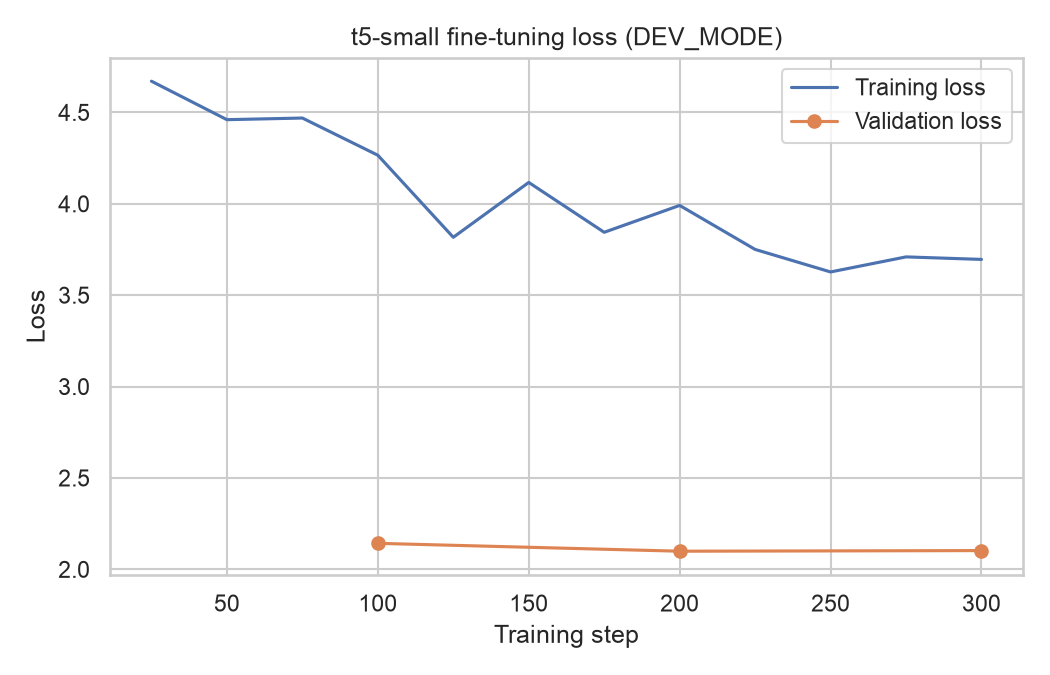
\includegraphics[width=0.8\textwidth]{figures/04_training_loss_curve.png}
    \caption{Training and validation loss during T5-small fine-tuning (confirmation run, 800 training pairs, three epochs).}
    \label{fig:training-loss}
\end{figure}

\chapter{Evaluation Methodology}
\label{ch:evaluation-methodology}

Every system in this project is judged from four different angles: whether the output reads as simpler, whether it overlaps with a human-written reference, whether it performs well on a metric built specifically for simplification, and whether it still means what the source sentence meant. No single metric covers all four questions, which is precisely why all of them are reported together rather than any one being treated as decisive. A manual reading of individual outputs, reported in \cref{ch:results-discussion}, is treated as a fifth and equally important check on all four.

\section{Readability Metrics}
\label{sec:readability-metrics}

Readability formulas estimate how difficult a passage is to read from surface features such as sentence length and syllable count. They say nothing about accuracy, but they are a fast, standard way to check whether an output looks simpler at all.

\subsection*{Flesch Reading Ease}

\begin{equation}
    \label{eq:flesch-reading-ease}
    FRE = 206.835 - 1.015 \left( \frac{\text{total words}}{\text{total sentences}} \right) - 84.6 \left( \frac{\text{total syllables}}{\text{total words}} \right)
\end{equation}

Scores range roughly from 0 to 100, with higher values indicating easier reading.

\subsection*{Flesch-Kincaid Grade Level}

\begin{equation}
    \label{eq:flesch-kincaid}
    FKGL = 0.39 \left( \frac{\text{total words}}{\text{total sentences}} \right) + 11.8 \left( \frac{\text{total syllables}}{\text{total words}} \right) - 15.59
\end{equation}

This approximates the US school grade level a reader would need to follow the text without difficulty.

\subsection*{SMOG Index}

\begin{equation}
    \label{eq:smog}
    SMOG = 1.0430 \sqrt{\text{polysyllable count} \times \dfrac{30}{\text{number of sentences}}} + 3.1291
\end{equation}

SMOG estimates the years of education needed to fully understand a passage, based on the number of words with three or more syllables.

\section{Overlap-Based Metrics}
\label{sec:overlap-metrics}

\subsection*{BLEU}

BLEU was originally designed for machine translation and measures $n$-gram overlap between a candidate and one or more references, adjusted by a brevity penalty that discourages overly short outputs~\cite{papineni2002bleu}.

\begin{equation}
    \label{eq:bleu}
    BLEU = BP \cdot \exp \left( \sum_{n=1}^{N} w_n \log p_n \right), \qquad BP = \min \left( 1,\ e^{1 - r/c} \right)
\end{equation}

Here $p_n$ is the modified $n$-gram precision, $w_n$ the weight assigned to that $n$-gram order, $r$ the reference length, and $c$ the candidate length.

\subsection*{ROUGE-N}

ROUGE measures recall-oriented $n$-gram overlap and is commonly used to check how much of a reference's content survives in a candidate text~\cite{lin2004rouge}.

\begin{equation}
    \label{eq:rouge}
    ROUGE\text{-}N = \frac{\displaystyle\sum_{S \in \text{Refs}} \sum_{\text{gram}_n \in S} \text{Count}_{\text{match}}(\text{gram}_n)}{\displaystyle\sum_{S \in \text{Refs}} \sum_{\text{gram}_n \in S} \text{Count}(\text{gram}_n)}
\end{equation}

This project reports ROUGE-1, ROUGE-2, and ROUGE-L, corresponding to unigram overlap, bigram overlap, and longest common subsequence overlap respectively.

\section{A Simplification-Specific Metric: SARI}
\label{sec:sari-metric}

BLEU and ROUGE were both built for tasks where staying close to the reference is the goal. Simplification is different, since a good rewrite is expected to remove some content and reword the rest, which a translation-style metric can penalise unfairly. SARI addresses this directly by scoring how well a system adds, keeps, and deletes $n$-grams relative to the source and the reference, rather than simply measuring overlap~\cite{xu2016sari}.

\begin{equation}
    \label{eq:sari}
    SARI = \frac{1}{3} \left( F_{\text{add}} + F_{\text{keep}} + P_{\text{delete}} \right)
\end{equation}

where $F_{\text{add}}$ and $F_{\text{keep}}$ are $n$-gram-level F1 scores for words correctly added and correctly retained, and $P_{\text{delete}}$ is the precision of words correctly removed, each averaged over $n$-gram orders one to four.

\section{Meaning Preservation: BERTScore}
\label{sec:bertscore-metric}

None of the metrics above can confirm that a simplified sentence still means what the source sentence meant. BERTScore addresses this by comparing candidate and reference text using contextual embeddings rather than exact word matches, so a paraphrase that uses different words can still score well if its meaning is close to the reference~\cite{zhang2020bertscore}.

\begin{equation}
    \label{eq:bertscore-p}
    P_{\text{BERT}} = \frac{1}{|\hat{x}|} \sum_{\hat{x}_j \in \hat{x}} \max_{x_i \in x} \mathbf{x}_i^{\top} \hat{\mathbf{x}}_j
\end{equation}

\begin{equation}
    \label{eq:bertscore-r}
    R_{\text{BERT}} = \frac{1}{|x|} \sum_{x_i \in x} \max_{\hat{x}_j \in \hat{x}} \mathbf{x}_i^{\top} \hat{\mathbf{x}}_j
\end{equation}

\begin{equation}
    \label{eq:bertscore-f1}
    F_{\text{BERT}} = 2 \cdot \frac{P_{\text{BERT}} \cdot R_{\text{BERT}}}{P_{\text{BERT}} + R_{\text{BERT}}}
\end{equation}

Here $x$ and $\hat{x}$ denote the token embeddings of the reference and candidate sentence respectively. This project reports BERTScore using \texttt{distilbert-base-uncased} as the underlying embedding model, a lighter alternative to the \texttt{roberta-large} model used in the original BERTScore paper, chosen to keep evaluation practical on the hardware available for this project.

\section{Qualitative Analysis}
\label{sec:qualitative-approach}

Automatic metrics are treated in this project as a starting point rather than a verdict. A manual reading of individual test examples was carried out alongside the automatic scores, chosen to represent a strong case, a neutral case, and a weak case for the fine-tuned model, using SARI and BERTScore as an initial filter before reading the actual text. This reading looks specifically for whether meaning was preserved, whether clinically relevant detail was lost, whether the output was simplified past the point of usefulness, and whether an output that scored well numerically actually reads as more natural or clear. \Cref{ch:results-discussion} reports what this reading found alongside the aggregate numbers.

\chapter{Results and Discussion}
\label{ch:results-discussion}

All four systems, the untouched source text, the heuristic baseline, zero-shot T5-small, and fine-tuned T5-small, were evaluated on the same random sample of 150 sentence pairs drawn from the Cochrane-auto test split. The human-written reference is included in the readability comparison as a point of reference, though overlap, simplification, and semantic similarity scores do not apply to it in the same way, since it is what the other systems are being compared against rather than a system in its own right.

\section{Automatic Metrics}
\label{sec:automatic-results}

\Cref{tab:readability-results} reports the three readability formulas for every system, and \cref{tab:generation-results} reports the overlap, simplification, and semantic similarity metrics for the three systems that produce a genuine rewrite.

\begin{table}[htbp]
    \centering
    \caption{Readability scores by system.}
    \label{tab:readability-results}
    \begin{tabular}{@{}lrrr@{}}
        \toprule
        \textbf{System} & \textbf{Flesch Reading Ease} & \textbf{Flesch-Kincaid Grade} & \textbf{SMOG} \\
        \midrule
        Source (unmodified)        & 26.72 & 14.55 & 15.33 \\
        Reference (human)          & 30.14 & 14.67 & 15.31 \\
        Heuristic baseline         & 29.53 & 14.04 & 14.84 \\
        Zero-shot T5-small         & 20.06 & 15.84 & 16.12 \\
        Fine-tuned T5-small        & 24.52 & 15.10 & 15.79 \\
        \bottomrule
    \end{tabular}
\end{table}

\begin{table}[htbp]
    \centering
    \caption{Overlap, simplification, and semantic similarity scores by system.}
    \label{tab:generation-results}
    \begin{tabular}{@{}lrrrrr@{}}
        \toprule
        \textbf{System} & \textbf{BLEU} & \textbf{ROUGE-1} & \textbf{ROUGE-L} & \textbf{SARI} & \textbf{BERTScore-F1} \\
        \midrule
        Source (unmodified)  & 29.59 & 0.553 & 0.497 & 51.94 & 0.881 \\
        Heuristic baseline   & 28.39 & 0.542 & 0.486 & 48.77 & 0.879 \\
        Zero-shot T5-small   & 19.31 & 0.366 & 0.327 & 36.29 & 0.787 \\
        Fine-tuned T5-small  & 29.81 & 0.561 & 0.505 & 50.50 & 0.885 \\
        \bottomrule
    \end{tabular}
\end{table}

\Cref{fig:metric-comparison} shows the same figures as a set of grouped bar charts, and \cref{fig:sari-vs-bertscore} plots SARI against BERTScore for each system, which makes the trade-off between simplification and meaning preservation easier to see at a glance than a table allows.

\begin{figure}[htbp]
    \centering
    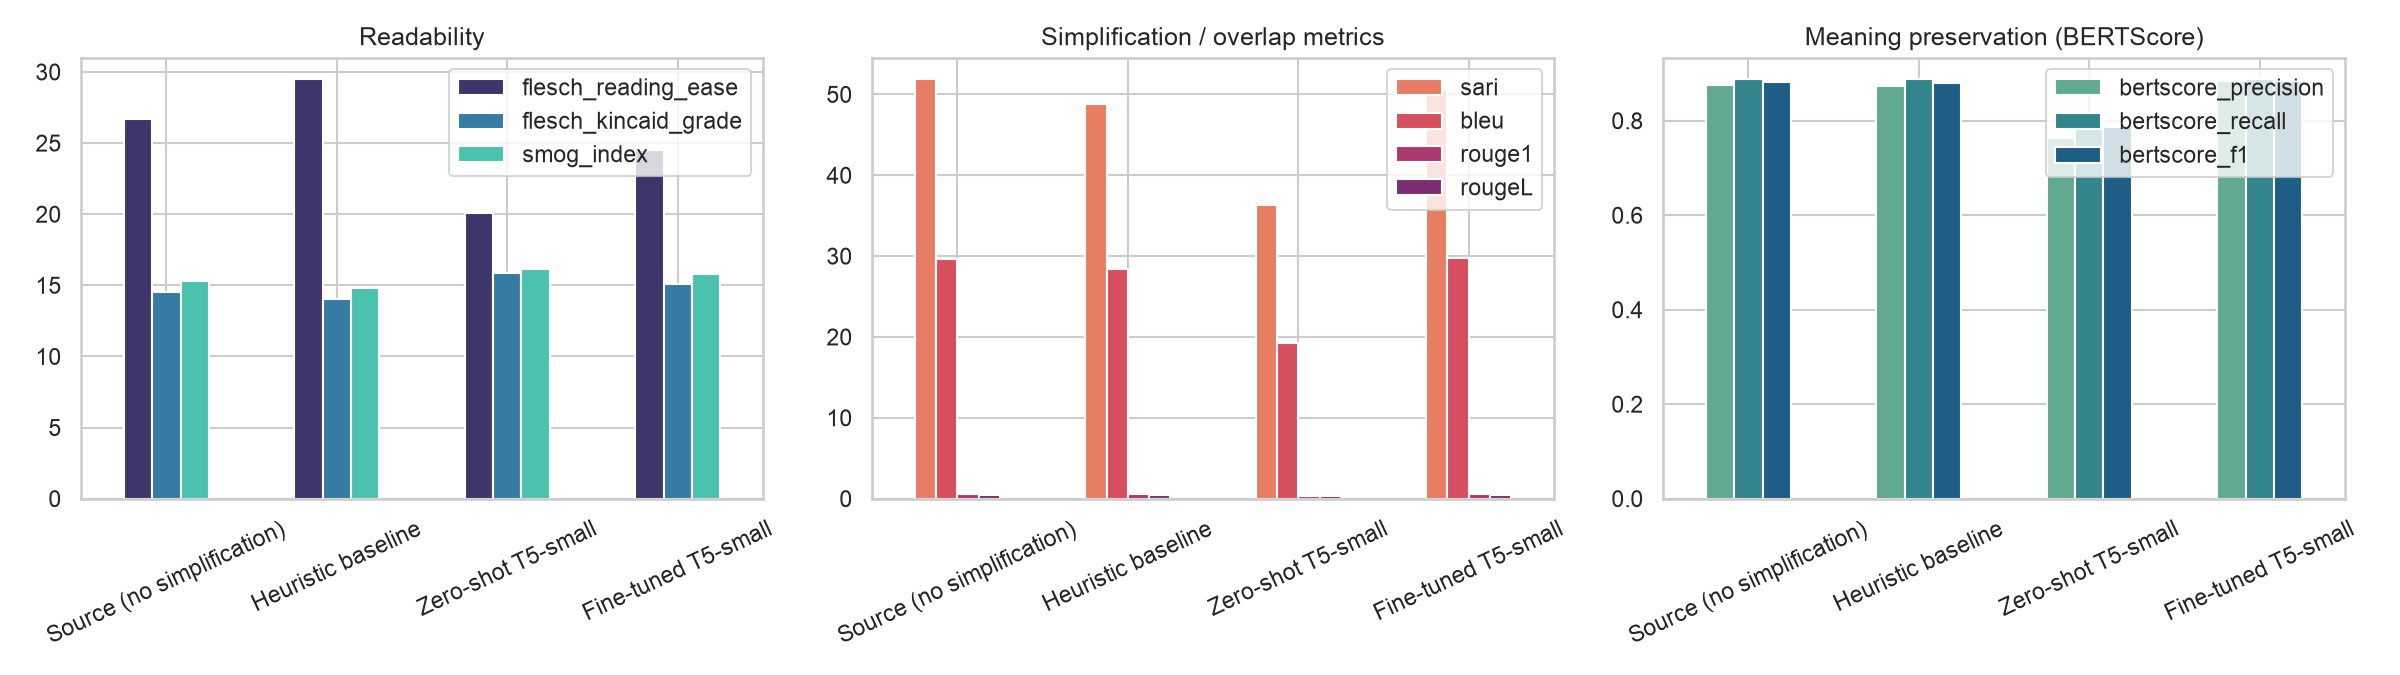
\includegraphics[width=\textwidth]{figures/05_metric_comparison.png}
    \caption{Readability, overlap, simplification, and meaning-preservation metrics across all four systems.}
    \label{fig:metric-comparison}
\end{figure}

\begin{figure}[htbp]
    \centering
    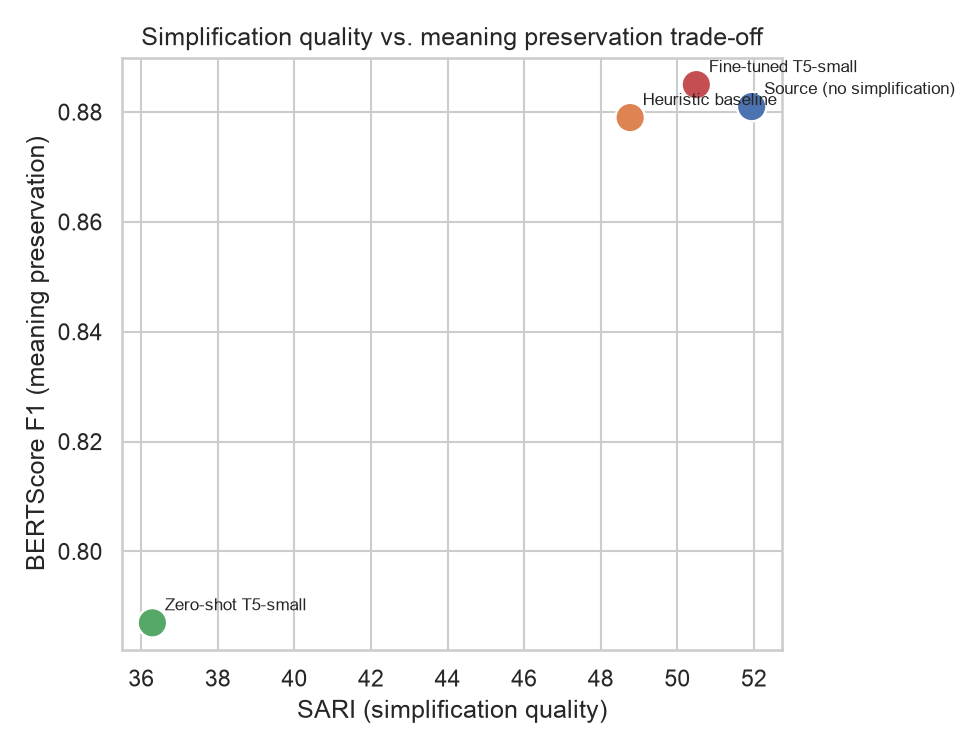
\includegraphics[width=0.75\textwidth]{figures/06_sari_vs_bertscore.png}
    \caption{SARI (simplification quality) against BERTScore F1 (meaning preservation) for each system.}
    \label{fig:sari-vs-bertscore}
\end{figure}

Two results stand out immediately. Fine-tuning made a clear difference relative to the untrained model. Zero-shot T5-small trails every other system on every metric by a wide margin, and a manual reading of its outputs explains why: without any exposure to the \texttt{"simplify: "} task on this data, the model frequently produced disfluent text or switched into a different language entirely rather than simplifying the input. Fine-tuning on only 800 examples for three epochs was enough to eliminate that failure mode completely and bring the model back to fluent, on-task English output.

Against the heuristic baseline, the comparison is closer and more informative. The fine-tuned model edges ahead on BLEU, ROUGE, and BERTScore, and very nearly matches the heuristic baseline's SARI score despite the heuristic system having been designed by hand specifically for this kind of sentence. On the readability formulas, however, the heuristic baseline actually scores slightly better than the fine-tuned model, and both trail the source text's own Flesch Reading Ease by less than might be expected for a system meant to simplify it. This is a genuine and honestly reported finding rather than an oversight, and \cref{sec:qualitative-discussion} explains what a manual reading of the outputs suggests is driving it.

\section{Qualitative Analysis}
\label{sec:qualitative-discussion}

Three examples were selected from the fine-tuned model's outputs on the test sample, one representing a clear success, one representing a partial or ambiguous result, and one representing a genuine failure to simplify. All three are reproduced here in full because the pattern they reveal matters more than any single score.

\subsection*{A Successful Simplification}

\begin{quote}
\textbf{Source:} ``One study with 59 teachers in 43 schools found no significant effects on job-related anxiety (MD -0.25 95\% CI -0.61 to 0.11, very low-quality evidence) or depression (MD -0.26 95\% CI -0.57 to 0.05, very low-quality evidence) after 24 months.''

\textbf{Fine-tuned output:} ``One study with 59 teachers in 43 schools found no significant effects on job-related anxiety or depression after 24 months.''
\end{quote}

The model removed both statistical parentheticals while keeping the claim itself intact and grammatically sound. This is close to the kind of edit the heuristic baseline was designed to make by hand, except the transformer produced it without an explicit rule telling it to strip confidence intervals. It is a genuine example of learned, rather than scripted, simplification behaviour.

\subsection*{A Neutral Case}

\begin{quote}
\textbf{Source:} ``Six RCTs with a total of 1211 participants were eligible; five trials evaluated oral aciclovir, and one, with 419 participants, evaluated oral famciclovir.''

\textbf{Reference:} ``They included a total of 1319 participants.''

\textbf{Fine-tuned output:} ``Six trials with a total of 1211 participants were eligible; five evaluated oral aciclovir, and one, with 419 participants, evaluated oral famciclovir.''
\end{quote}

The model made only a small lexical change here, replacing ``RCTs'' with ``trials,'' while the human reference summarised the same information in a completely different and much shorter way. Notice also that the reference states a participant count, 1{,}319, that does not match the 1{,}211 given in the source sentence. That discrepancy appears to be a genuine inconsistency in the original Cochrane materials rather than a modelling error, and it is a useful reminder that not every gap between a model's output and its reference reflects a failure of simplification. Sometimes it reflects noise already present in the training data, which is worth flagging for anyone extending this work.

\subsection*{A Failure Case}

\begin{quote}
\textbf{Source:} ``We identified only low- or very low-certainty evidence to judge the effectiveness of inhaled antibiotics for the treatment of pulmonary exacerbations in people with cystic fibrosis.''

\textbf{Reference:} ``We graded the certainty of the evidence as very low or low.''

\textbf{Fine-tuned output:} \textit{(identical to the source, no change made)}
\end{quote}

Here the model made no edit at all, while the reference restructures the sentence almost completely, dropping the specific clinical context and restating only the certainty judgement. This is the clearest evidence in the results that, at the training scale used for this confirmation run, the model has learned to make small, local edits such as deleting a clause or swapping a word, but has not yet learned the kind of deeper restructuring a human writer uses when a sentence needs more than light editing. That is a limitation of scale rather than of the approach itself, and \cref{ch:conclusion} discusses what a longer training run on the full dataset would be expected to change.

\section{Discussion}
\label{sec:discussion}

Read together, these results support a specific and fairly narrow conclusion rather than a sweeping one. Fine-tuning a small transformer on domain-specific aligned data clearly teaches it to behave sensibly on this task, where the same model without fine-tuning does not. It also modestly outperforms a hand-built heuristic on the metrics designed specifically for simplification and meaning preservation, SARI and BERTScore, while trailing that same heuristic slightly on surface readability. The most likely explanation, based on the manual reading above, is that this confirmation run's small training set and short schedule taught the model a conservative editing strategy rather than the more substantial restructuring that both the heuristic rules and the human reference summaries sometimes apply. That the heuristic baseline can compete with, and in one respect beat, a fine-tuned transformer is itself a useful finding. It suggests that at least part of what makes Cochrane lay summaries easier to read, removing dense statistical detail, is learnable by hand-written rules almost as well as by a trained model, at least at this scale of training.

This chapter's results also revisit a point raised in \cref{ch:dataset}: a meaningful share of the reference summaries do more than compress their source sentence, sometimes adding context, sometimes restating a different but related fact, and occasionally, as in the aciclovir example above, containing an inconsistency that has nothing to do with simplification quality at all. Any evaluation of this task needs to hold that in mind before treating a lower automatic score as straightforward evidence of a weaker model.

\chapter{Conclusion}
\label{ch:conclusion}

\section{Summary of Contributions}
\label{sec:summary-contributions}

This project set out to answer a narrow but practical question: can a transformer-based model simplify public-facing health information without quietly losing the meaning that makes the information useful in the first place. The answer, on the evidence gathered here, is a qualified yes. A T5-small model fine-tuned on Cochrane-auto produces fluent, on-task simplifications where the same model without fine-tuning frequently does not, and it modestly outperforms a hand-written rule-based baseline on the metrics built specifically to measure simplification quality and meaning preservation. It does not yet outperform that same baseline on every measure, and a manual reading of individual outputs suggests why: at the training scale used for the confirmation run reported in \cref{ch:results-discussion}, the model has learned to make small, safe edits rather than the deeper restructuring that some sentences genuinely need.

Beyond the specific numbers, this project produced a working, documented, and reproducible pipeline covering dataset preparation, two baselines, a fine-tuning procedure, and a five-part evaluation combining readability formulas, overlap metrics, a simplification-specific metric, a semantic similarity measure, and a manual reading of outputs. Every design choice, including ones that reduced surface performance, such as declining to strip statistical detail in the heuristic baseline, was made deliberately and is documented in this thesis rather than left implicit.

\section{Limitations}
\label{sec:limitations}

The results in this thesis come from a confirmation run using 800 of the 7{,}075 available training pairs over three epochs, run on hardware without a dedicated GPU. This was a deliberate choice made to validate that the full pipeline behaves correctly end to end before committing to a longer run, and the thesis has been explicit throughout about which numbers come from this smaller run rather than presenting them as the final word on the model's ability. A full run over the complete training set for up to eight epochs is the natural next step, and \cref{sec:future-work} sets out what would change as a result.

The evaluation itself has narrower limitations too. BERTScore was computed using \texttt{distilbert-base-uncased} rather than the larger \texttt{roberta-large} model used in the original BERTScore paper, a choice made for practicality on the available hardware that may understate meaning-preservation scores slightly. The qualitative analysis in \cref{ch:results-discussion} examined three illustrative examples in detail rather than a large systematic sample, which is enough to identify a pattern but not enough to quantify how often that pattern occurs across the full test set. Finally, this project works entirely at sentence level, which sidesteps the document-level coherence questions raised in \cref{sec:variation-coherence} and leaves them open for future work.

\section{Ethical Considerations}
\label{sec:ethics}

This project uses only publicly available datasets, Cochrane-auto, ASSET, and WikiAuto, and involves no direct interaction with patients or clinical data. Even so, the application it points toward carries real ethical weight. A simplification model can produce text that reads as authoritative and clear while quietly dropping a limitation, a condition, or a note of uncertainty that a clinician would consider essential. It can also, in the opposite direction, make a claim sound more certain than the evidence actually supports, simply by replacing careful, hedged scientific language with a more direct sentence. Both risks were treated as central design concerns throughout this project rather than as an afternote, which is why meaning preservation was evaluated with the same seriousness as readability rather than as a secondary check.

This system is not positioned, and should not be read, as a medical decision-making tool. It is an assistive drafting aid at most, intended to sit alongside human review rather than replace it. The failure case examined in \cref{sec:qualitative-discussion}, where the model made no edit at all to a sentence that needed substantial rewriting, is arguably a safer failure mode than the alternative of confidently producing a fluent but inaccurate simplification, and that asymmetry is worth keeping in mind when judging what counts as an acceptable error rate for a system like this one.

\section{Future Work}
\label{sec:future-work}

Several extensions follow directly from the limitations above. The most immediate is completing a full training run across all 7{,}075 training pairs for up to eight epochs, which the pipeline already supports and which would give a fairer picture of what fine-tuning at this scale can achieve. Repeating the same pipeline with BART-base, noted throughout this thesis as an alternative architecture, would show whether the results reported here are specific to T5-small or hold more generally across compact transformer models. Re-running BERTScore with \texttt{roberta-large} would bring the meaning-preservation evaluation in line with the original metric's recommended configuration.

Beyond these direct extensions, two questions raised earlier in this thesis remain genuinely open. The dataset analysis in \cref{ch:dataset} suggested that a meaningful share of Cochrane lay summaries add explanatory content rather than simply compressing their source sentence, which points toward framing this task, at least in part, as constrained lay summarisation rather than sentence-level simplification in the narrow sense. A future iteration of this project could test that framing directly by training on paragraph-level or document-level pairs rather than isolated sentences. The coherence concerns raised in \cref{sec:variation-coherence} point in the same direction. A patient information document is read as a connected argument, not as a set of independently simplified sentences, and evaluating a health simplification system at document level would be a natural and worthwhile continuation of the work presented here.


% ----------------------------------------------------------------------
% References -- IEEE numeric style
% ----------------------------------------------------------------------
\bibliographystyle{ieeetr}
\bibliography{references}

\end{document}
